\documentclass[11pt,reqno]{amsart}
\usepackage[top=1in, left=1in, right=1in, bottom=1in]{geometry}                % See geometry.pdf to learn the layout options. There are lots.
\geometry{letterpaper}                   % ... or a4paper or a5paper or ...
\usepackage[parfill]{parskip}    % Activate to begin paragraphs with an empty line rather than an indent

\usepackage{algorithm}
\usepackage{algpseudocode}
\usepackage{hyperref}
\usepackage{graphicx}
\usepackage{url}
\usepackage{verbatim}
\usepackage{amssymb}
\usepackage{amsaddr}
\usepackage{amsmath}
\usepackage{enumitem}
\usepackage{setspace}
\usepackage{natbib}
\usepackage{booktabs}

\newcommand{\RR}{I\!\!R} %real numbers
\DeclareMathOperator{\diag}{diag}

\algnewcommand{\Inputs}[1]{%
  \State \textbf{Inputs:}
  \Statex \hspace*{\algorithmicindent}\parbox[t]{.8\linewidth}{\raggedright #1}
}
\algnewcommand{\Initialize}[1]{%
  \State \textbf{Initialize:}
  \Statex \hspace*{\algorithmicindent}\parbox[t]{.8\linewidth}{\raggedright #1}
}


\title[Reveiw on RVD Methods]{Review on rare genetic variant detection methods for next-generation sequencing data}
\author[F. Zhang AND P. Flaherty]{Fan Zhang\,$^{1}$, Patrick Flaherty\,$^{1,2}$}
\address{$^{1}$Department of Biomedical Engineering, Worcester Polytechnic Institute, MA, USA\\
$^{2}$Department of Mathematics and Statistics, University of Massachusetts, Amherst, MA, USA}

\begin{document}
\maketitle

\section{Introduction}
%\subsection{Sequence Analysis Pipeline}
%Scope of the article: nucleotides and variant calling in the context of larger pipeline.
Next-generation sequencing (NGS) technology has revealed the presence of extensive genomic variants in clinical samples.
In general, genomic variants can be present in the form of single nucleotide variants (SNVs), insertions and deletions, structural variants, and copy number variations.
Single nucleotide variant is a primary source of genetic variation that can cause susceptibility to disease or drug resistance to  anti-tumour therapeutics.
The general pipeline to analyze single nucleotide variants in the large-scale NGS data basically consists five main steps: quality control, preprocessing, alignment, post-alignment processing, and variant analysis ~\citep{Bao2014}.
Variant analysis basically contains three main parts: variant detection, annotation, and visualization, among which variant detection is crucial for NGS data analysis with an objective of discovering disease-causing variants.
In this review, we focus on single nucleotide variant detection in DNA next-generation sequencing data and classification of current computational and statistical variant detection methods.

%Outline the paper here with one paragraph overview per section.
We first highlight the necessity of a sensitive variant detection method from the perspective of biological impacts and statistical accuracy,
and then present the hallmarks of a good variant detection method based on the evaluation of accuracy, scalability, and robustness.
We also discuss the issues that will effect the ability of variant detection methods.
Finally, we classify the state-of-the-art variant detection methods into the categories of probabilistic and non-probabilistic methods and survey each method in detail.


\section{Why do we need a sensitive variant detection method?}

\subsection{Motivation}
Most variants are revealed to be rare by 1000 Genomes ~\citep{10002010map} and rare variants do cause risk of disease or have large effects ~\citep{kosmicki2016discovery}.

\subsection{Biological impacts}


\subsection{Statistical accuracy}
Since the allele frequency of rare variants is low, it needs high statistical power to identify rare variants especially when the sample size is not large.

What is the payoff for spending time and energy on this problem.



%\subsection{Variants}
%\subsubsection{Germline, somatic, or LOH (loss of heterozygosity)}
%\subsubsection{Rare and common variants}

\section{Hallmarks of a good variant detection method}
\subsection{Accuracy}

\subsection{Scalability}

\subsection{Robustness}

Tradeoff between accuracy and scalability.

It depends on specific purposes.

\section{Factors that affect the ability of variant detection methods}
The next-generation sequencing data is massive and heterogeneous and many factors could influence the performance of a variant detection method.
\subsection{Quality control}
The quality of the data can affect variant detection, so checking the quality of the raw data and filtering the low-confidence alleles in advance will improve the accuracy of variant detection.
A standard tool, FastQC, is implemented for assessing the quality by generating analytical graphs.
Low-confidence alleles can be trimmed using a standalone tool, NGS QC Toolkit ~\citep{patel2012ngs}, to prevent from making a wrong variant call.
Although filtering low-confidence alleles helps with read alignment, it is noticeable that false positives could be introduced for high-coverage data set ~\citep{liu2012steps}.
Thus, we should consider not only quality control in read mapping but also the read depth of coverage in order to ensure the accuracy of variant detection.

\subsection{Depth of coverage}
Sequencing depth of coverage, number of times that each base has been sequenced, contributes to the results of variant detection because sufficient depth of coverage is necessary to support an accurate variant call.
Due to the high cost of sequencing, the depth of coverage of the sequencing data can be low (less than $10\times$) and the distribution of the read depth over each site could be not uniform.
Previous researchers have studied the effect of coverage and revealed that high coverage data leads to high sensitivity of variant detection ~\citep{neuman2013analysis, krawitz2010microindel}.
~\citep{liu2013variant} indicates that the false discovery rate of variant detection using GATK decreased as the depth of coverage increased.
Generally, the minimum coverage for a single nucleotide polymorphism is 50x and some applications may need higher coverage ~\citep{Schlotterer2014}.
It is reasonable that if you desire to detect a rare variant of $0.1 \%$ allele frequency, the required depth of coverage i $1000\times$.
Furthermore, unmatched sequencing read depths of case and control samples will result in increased false positives ~\citep{garner2011confounded}.
%Develop probabilistic methods to estimate the posterior probability of each site to be a variant in the low read depth data.

\subsection{Sequencing errors}
Intrinsic errors from next-generation sequencing platform exist in sample processing and sequencing ~\citep{Olson2015}.
These errors may cause false positives and false negatives in the variant detection step.
Especially, identification of variants of minor variant allele frequency (VAF) is challenging because it is difficult to differentiate a true rare variant (VAF $<$1 \%) from a common sequencing error rate (1\% $<$ VAF $<$ 3\%).
% give an example error from sample processing
% give an example error from sequencing
% give an example error from variant detection
In variant detection step, errors may also exist due to the limitation of the design of the variant detection methods.
For example, a prior assignment in a probabilistic method can be subjective, which may cause bias to predict the probabilistic distribution of the allele frequency of a site in the sequence.
This will lead a miscalling of a rare variant when comparing the allele frequencies of one site in a control/case pair.

\subsection{Sample size}
Multiple samples (pooled sequencing) enabled us to identify more rare variants than individual sample ~\citep{Bao2014, liu2012steps}.
~\citep{liu2013variant} demonstrated that GATK gives higher sensitivity for variant detection in a multiple-sample strategy than a single-sample strategy, but the specificity turned out to be decreased in multiple-sample strategy.
The reason is that more false positives are called in larger data sets with multiple samples ~\citep{Nielsen2011}.
However, if the coverage of the multiple samples is low, the false discovery rate for variant detection could be increased compared with the case of high coverage ~\citep{Cheng2014}.
~\citep{le2011snp} observed that large data set of multiple sequencing samples at low coverage (4-6$\times$) yields higher capability in rare variant detection compared to small data set of less sequencing samples at high coverage.

\section{Classification for variant detection methods}
We classify the state-of-the-art variant detection methods into two categories - probabilistic methods, and non-probabilistics or other combination (Table \ref{tbl:methods}).
We discuss every method from three aspects: specific purpose of the method, category that this method falls into, and metrics or its applications.

%\begin{table}[htbp]
%\centering
%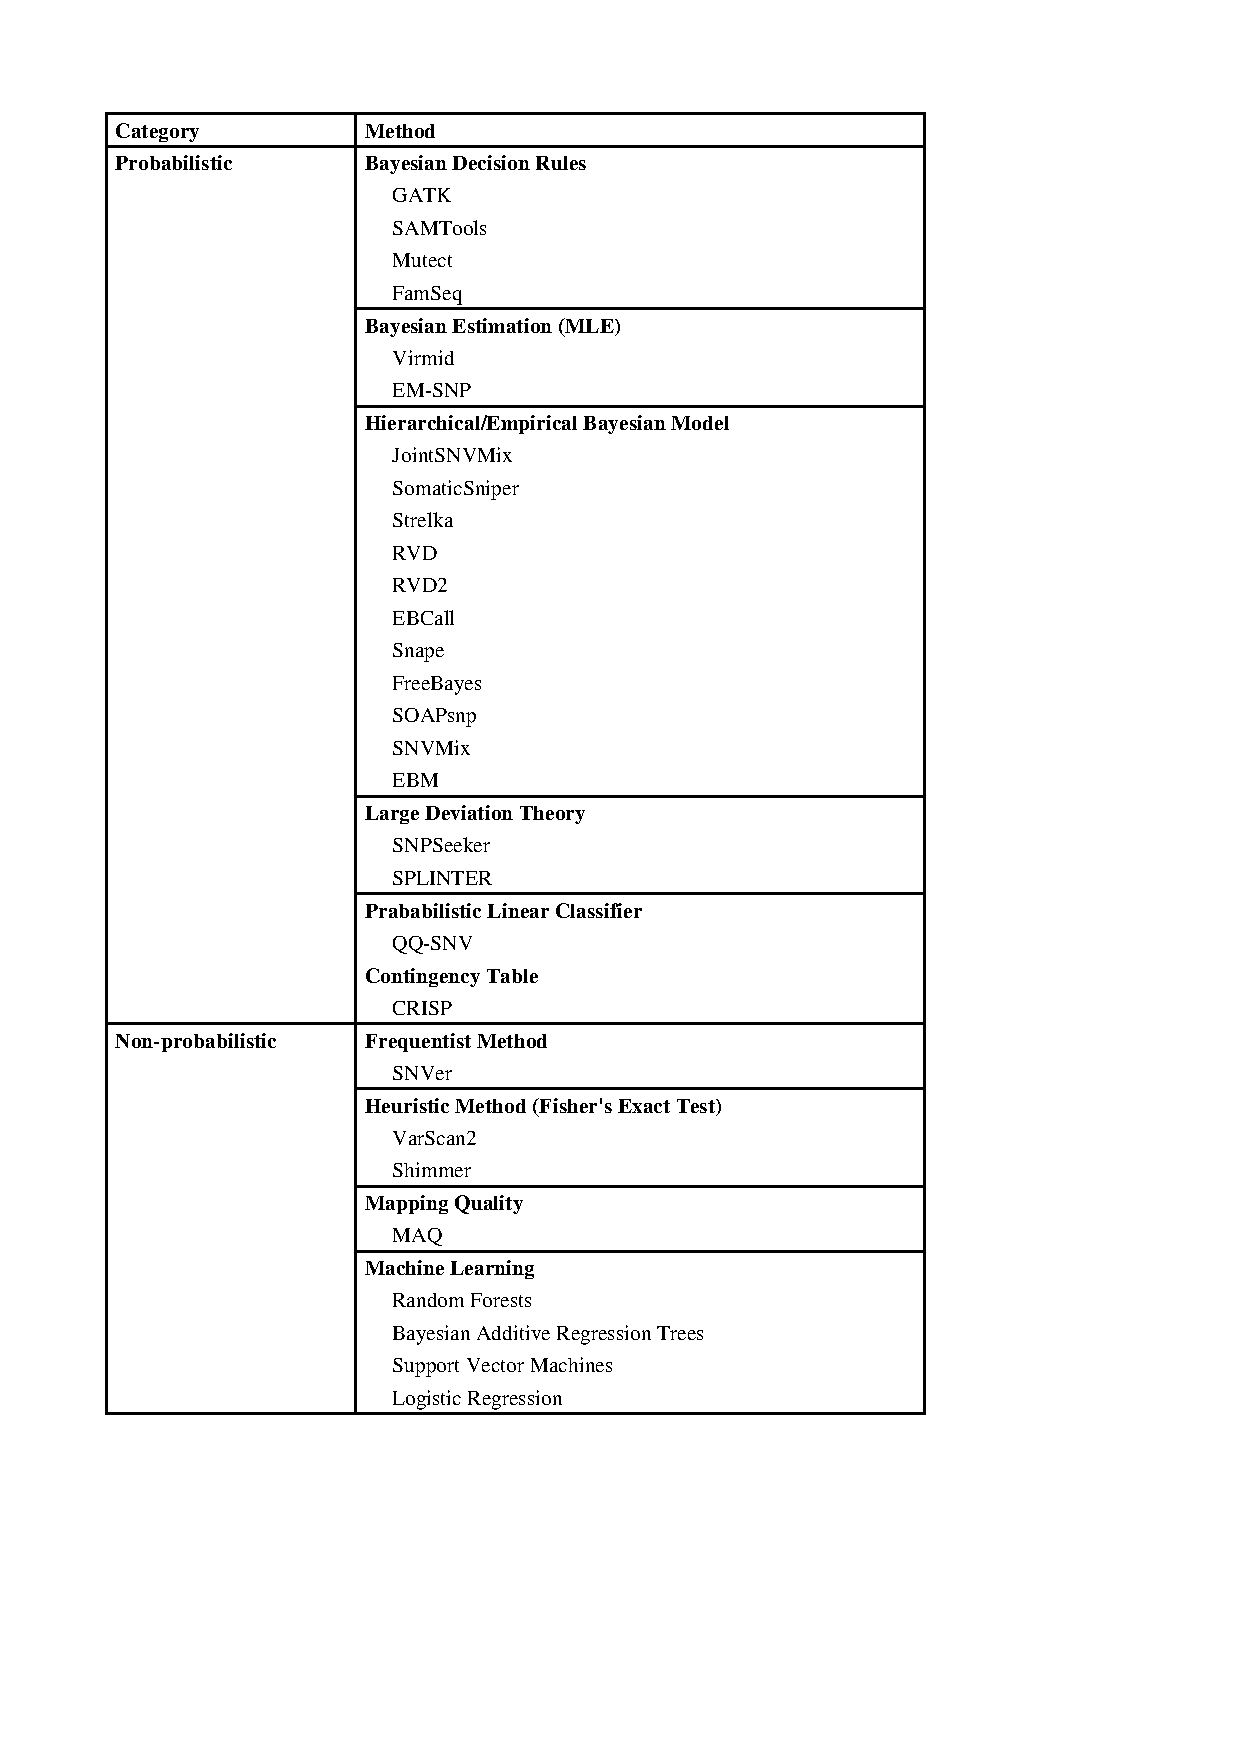
\includegraphics[width=0.9\textwidth]{method_table.pdf}
%\caption{Single nucleotide variant detection methods.}
%\label{tbl:methods}
%\end{table}

\begin{table}[htbp]
  \centering
  \caption{Classification of variant detection methods in next-generation sequencing data.}\label{tbl:methods}
  \footnotesize
    \begin{tabular}{rr}
    \toprule
    \textbf{Category} & \multicolumn{1}{l}{\textbf{Method}} \\
    \midrule
    \textbf{Probabilistic} & \multicolumn{1}{l}{\textbf{Bayesian Decision Rules}} \\
          & \multicolumn{1}{l}{GATK} \\
          & \multicolumn{1}{l}{SAMTools} \\
          & \multicolumn{1}{l}{Mutect} \\
          & \multicolumn{1}{l}{FamSeq} \\
          & \multicolumn{1}{l}{\textbf{Bayesian Estimation}} \\
          & \multicolumn{1}{l}{ Virmid} \\
          & \multicolumn{1}{l}{ EM-SNP} \\
          & \multicolumn{1}{l}{\textbf{Hierarchical/Empirical Bayesian Model}} \\
          & \multicolumn{1}{l}{JointSNVMix} \\
          & \multicolumn{1}{l}{SomaticSniper} \\
          & \multicolumn{1}{l}{Strelka} \\
          & \multicolumn{1}{l}{RVD} \\
          & \multicolumn{1}{l}{RVD2} \\
          & \multicolumn{1}{l}{Variational RVD} \\
          & \multicolumn{1}{l}{EBCall} \\
          & \multicolumn{1}{l}{Snape} \\
          & \multicolumn{1}{l}{FreeBayes} \\
          & \multicolumn{1}{l}{Seurat} \\
          & \multicolumn{1}{l}{SOAPsnp} \\
          & \multicolumn{1}{l}{SNVMix} \\
          & \multicolumn{1}{l}{EBM} \\
          & \multicolumn{1}{l}{\textbf{Large Deviation Theory}} \\
          & \multicolumn{1}{l}{SNPSeeker} \\
          & \multicolumn{1}{l}{SPLINTER} \\
          & \multicolumn{1}{l}{\textbf{Prababilistic Linear Classifier }} \\
          & \multicolumn{1}{l}{QQ-SNV} \\
          & \multicolumn{1}{l}{\textbf{Contingency Table }} \\
          & \multicolumn{1}{l}{CRISP} \\
          \midrule
    \textbf{Non-probabilistic} & \multicolumn{1}{l}{\textbf{Frequentist Method}} \\
    \textbf{Other combination} & \multicolumn{1}{l}{SNVer} \\
         & \multicolumn{1}{l}{\textbf{Heuristic Method}} \\
         & \multicolumn{1}{l}{VarScan2} \\
         & \multicolumn{1}{l}{Shimmer} \\
         & \multicolumn{1}{l}{\textbf{Mapping Quality}} \\
         & \multicolumn{1}{l}{MAQ} \\
         & \multicolumn{1}{l}{\textbf{Machine Learning}} \\
         & \multicolumn{1}{l}{Atlas2} \\
         & \multicolumn{1}{l}{Random Forests} \\
         & \multicolumn{1}{l}{Bayesian Additive Regression Trees} \\
         & \multicolumn{1}{l}{Support Vector Machines} \\
         & \multicolumn{1}{l}{Logistic Regression} \\
    \bottomrule
    \end{tabular}
\end{table}


\subsection{Probabilistic Methods}
We summary 21 variant detection methods that are developed based on probabilistic strategy in detail.

GATK ~\citep{McKenna2010} is designed for detecting germline variants in homogeneous samples.
It uses a simple Bayesian genotyper to calculate the posterior distribution of each genotype given mapped reads over each site ~\citep{depristo2011framework}.
It adopted a MapReduce system to facilitate processing large-scale sequencing data in parallel and has been involved in 1000 Genomes Project and The Cancer Genome Atlas.

SAMtools ~\citep{Li2009a} is implemented to manipulate the genomic sequences in the SAM and BAM format.
Similar to GATK, SAMtools computes the likelihood of each possible genotype using a naive Bayesian model and then identifies germline variants using BCFtools ~\citep{li2011statistical}.
It has been demonstrated for comparable accuracy in real data for allele count estimation, allele frequency estimation, and association mapping.

MuTect ~\citep{Cibulskis2013} is a method to detect germline and somatic variants with low allele frequencies at various sequencing read depths in mixed tumour samples.
It is built on a Bayesian classifier to calculate a log-likelihood ratio that can be used as a threshold for variant detection in matched tumour and normal samples.
It has been shown that MuTect is more sensitive than other competing methods in detecting somatic variants within low fraction of tumour cells, which enables us to discover subclonal drivers for tumour progression.

SomaticSniper ~\citep{Larson2012} detects somatic variants by directly comparing the joint diploid genotype likelihoods for a tumour-normal pair.
The genotype likelihood is calculated using MAQ method ~\citep{Li2008} by  incorparating the dependency of the genotypes between tumour and normal samples.
Sensitivity and precision are employed to evaluate the performance of variant detection on a simulated data set.

Strelka ~\citep{Saunders2012} is an algorithm for somatic variant detection in a joint analysis of matched tumour and normal samples.
It is a Bayesian method that models the joint probabilistic distribution of continuous allele frequencies.
Strelka is capable to maintain high sensitivity in low purity tumour samples.

JointSNVMix ~\citep{Roth2012} is introduced to discover somatic point variants and distinguish germline from somatic events.
It applies two novel Bayesian probabilistic models to jointly analyze the allelic count of tumour and normal samples.
Concordance is used as a probabilistic threshold to measure the performance of variant detection.
Is has been demonstrated that the joint modelling, JointSNVMix, has higher specificity than its independent analogue with guaranteed sensitivity.

Virmid ~\citep{Kim2013} is implemented for somatic variant detection using the idea of estimating the level of sample contamination.
Maximum likelihood estimation is used for sample impurity estimation and joint genotype probability estimation, and Bayesian inference is used for variant detection.
The strategy of estimating the level of contamination helps to reduce computational running time and increase accuracy in variant detection.

FreeBayes ~\citep{Garrison2012} is a haplotype-based variant detection method for short read DNA sequencing data.
It is a generalization of a Bayesian statistical method ~\citep{marth1999general} to detect variants in both individual and pooled samples.
A gradient ascent method is employed to establish a maximum a posteriori (MAP) estimate of the genotype for each sample.
This framework is able to identify longer and multi-alleles by modelling multiallelic site.

CRISP ~\citep{Bansal2010} method identifies both rare and common variants in pooled sequencing samples.
It is a probabilistic method that computes a contingency table P-value and a quality-based P-value that represent the probability of the absence of a variant and can then be used to differentiate true variants from sequencing errors.
CRISP is able to detect a 2\% allele frequency event in a dataset of two pools with 25 individuals each.

EBCall ~\citep{Shiraishi2013} is proposed to detect somatic variants by incorporating sequencing errors as prior information into the model.
It is developed based on an empirical Bayesian framework where Beta-Binomial distribution is used to depict sequencing errors.
EBCall can detect somatic variants of less than 10\% allele frequencies in tumour subclones.

FamSeq ~\citep{Peng2013} is a family-based sequencing program for variant detection in the data of family members.
FamSeq uses Bayesian network to yield posterior probabilities for measure of genotype calls and MCMC sampling method to derive the posterior probabilities.
This method integrates Mendelian inheritance and sequencing data of family members to reduce the false positive rate and false negative rate for variant detection.

EM-SNP ~\citep{Chen2013} can be used for allele frequency estimation, SNVs detection and association study in pooled sequencing data.
They developed an expectation maximization (EM) algorithm to approximate the maximum likelihood of the parameters to estimate the minor allele frequencies.
It has been shown that EM-SNP outperforms SNVer in rare variants detection in the type 1 diabetes pooled sequencing data by comparison on the metrics of dbSNP and transition/transversion ratio.

Snape ~\citep{Raineri2012} is built to detect SNVs in pooled samples.
It is a Bayesian method that takes into account of different priors to estimate the posterior frequency probability of SNVs.
Snape has low false discovery rate and high power on a simulated data set that is generated by ART ~\citep{huang2012art}.

SOAPsnp ~\citep{Li2009} is a variant detection method that is designed for massively parallel sequencing-by-synthesis Illumina Genome Analyzer data.
It uses a Bayesian statistical model to infer the likelihood of each possible genotype and outputs the genotype with highest posterior proabability for each site.
it achieves high accuracy in a human genome deep resequencing data and incorparating dbSNP genotypes as prior information helps with identify real heterozygotes in low read depth data.

SNVMix ~\citep{Goya2010},

EBM ~\citep{Zhou2012},

SNPSeeker ~\citep{Druley2009},

SPLINTER ~\citep{Spencer2014},

QQ-SNV ~\citep{VanderBorght2015},

Seurat ~\citep{Christoforides2013} aims to detect somatic events, including SNVs, insertion/deletions, and structural variations, within tumors in paired tumor and normal samples.
Seurat is a generalized Bayesian framework that uses a beta-binomial distribution to model the probability of a somatic event.
Seurat shows high transition/transversion ratio, low non-synonymous/synonymous ratio, and low dbSNP rate on a lymphoma tumor data set, which demonstrates that Seurat has high specificity.

DeepSNV ~\citep{gerstung2012reliable} is a powerful statistical method for detecting SNVs in ultra-deep sequencing data.
This algorithm is built on a hierarchical beta-binomical model and a likelihood ratio test is calculated for each base for comparison with a control or a reference.
DeepSNV is validated on subclonal diverse tumour samples of renal cell carcinoma and reveals an agreement of the variant allele frequencies of the variants with the original work ~\citep{gerstung2012reliable}.

We previously developed a Beta-Binomial model, RVD ~\citep{Flaherty2012}, to characterize error rate distribution of each site of the next-generation sequencing data.
RVD is able to detect a 0.1\% variant allele frequency event in a synthetic DNA data set.
Then, we developed RVD2 ~\citep{He2015} that improved RVD by adding priors to tie parameters across sites and derived a Markov Chain Monte Carlo (MCMC) sampling algorithm for posterior inference.
Based on this improvement, RVD2 can handle low read depth sequencing data and manipulate multiple replicates.
Furthermore, we proposed a variational expectation maximization algorithm ~\citep{zhang2016variational} for the Bayesian statistical model to detect single nucleotide variants in heterogeneous samples.
Variational EM algorithm is demonstrated with comparable sensitivity and specificity compared with other state-of-the-art algorithms and can track non-reference allele frequency in a real time-series sequencing data set


\subsection{Non-probabilistic Methods}
We summary 6 variant detection methods that are developed based on non-probabilistic or other combination methods.

SNVer ~\citep{Wei2011} is a common and rare variant detection method for both individual and pooled sequencing data and it is scalable for whole genome sequencing data.
This is a frequentist method that reports overall P-values for every site without discarding bases with low read depth.
Transition and transversion ratio, genotype concordance, and dbSNP are metrics for evaluating the quality of variant calls in a real pooled sequencing data application ~\citep{depristo2011framework}.

VarScan2 ~\citep{Koboldt2012} is published for detecting somatic variants, loss of heterozygosity, and germline variants in exome sequencing data.
% "It also detects copy number variants but it is not related with our topic."
VarScan2 uses a heuristic method and a Fisher's exact test by comparing tumour and normal samples based on several thresholds, such as the number of allele counts and variant allele frequency.
In a test of 151 ovarian tumour samples from TCGA data set, it identified 7,790 validated somatic variants with 93\% sensitivity and 85\% precision.

Shimmer ~\citep{Hansen2013} is a method to identify somatic changes in normal-tumor samples.
It uses Fisher's exact test with Benjamini-Hochberg ~\citep{benjamini1995controlling} for multiple testing correction to control the false discovery rate (FDR).
Its advantage is to be sensitive to detect variants in highly heterogeneous tumor data.

Atlas2 ~\citep{challis2012integrative} aims to detect SNVs in the whole exome sequencing (WES) data from the platforms of SOLiD, Illumina, and Roche 454.
Atlas2 uses a logistic regression model to detect SNVs that pass the heuristic filters.
It has been integrated into the Genboree for easily processing the next-generation sequencing data on a web-based platform.

MAQ ~\citep{Li2008},

Random Forests ~\citep{Ding2012},
Bayesian Additive Regression Trees ~\citep{Ding2012},
Support Vector Machines ~\citep{Ding2012},
Logistic Regression ~\citep{Ding2012}.


\bibliography{bib}
\bibliographystyle{named}
\end{document}
